\documentclass[arhiv]{../izpit}
\usepackage{fouriernc}
\usepackage{xcolor}
\usepackage{tikz}
\usepackage{fancyvrb}
\usetikzlibrary{calc,shapes.multipart,chains,arrows,fit,shapes}
\VerbatimFootnotes{}


\begin{document}
	
	\izpit{Programiranje I: 2. izpit}{10.\ februar 2020}{
		Čas reševanja je 150 minut.
		Veliko uspeha!
	}
	
	%%%%%%%%%%%%%%%%%%%%%%%%%%%%%%%%%%%%%%%%%%%%%%%%%%%%%%%%%%%%%%%%%%%%%%%

	\naloga 
  
	\podnaloga Napišite funkcijo za izračun skalarnega produkta dveh vektorjev iz $\mathbb{R}^3$.
  \begin{verbatim}
    dot_prod: float * float * float -> float * float * float -> float
  \end{verbatim}

  \podnaloga Napišite funkcijo višjega reda, ki sprejme funkcijo dveh argumentov in drugi argument fiksira na podano vrednost. 
  \begin{verbatim}
    fix_second : ('a -> 'b -> 'c) -> 'b -> 'a -> 'c
  \end{verbatim}

	\podnaloga Napišite funkcijo \verb|combine_and_filter f xs ys|, kjer imajo argumenti tipe \verb|xs : 'a list|, \verb|ys : 'b list| in \verb|f : ('a -> 'b -> 'c option)| ter vrne vrednost tipa \verb|'c list|. Funkcija istoležne elemente seznamov preslika z \verb|f| in vrne seznam vseh smiselnih rezultatov. Če seznama nista iste dolžine, se izvaja zgolj do konca krajšega od seznamov. Za vse točke naj bo repno rekurzivna.
	\begin{verbatim}
  # let safe_minus x y = if x > y then Some (x-y) else None
    combine_and_filter safe_minus [1;0;4;3] [2;1;0;2;5];;
  - : int list = [4; 1]
	\end{verbatim}
	
	\podnaloga Napišite funkcijo, ki sprejme predikat in seznam nizov in izpiše z vejico ločene elemente seznama, za katere predikat velja. Pazite, da bo tip funkcije pravilen.
  \begin{verbatim}
  # conditional_print;;
  - : (string -> bool) -> string list -> unit = <fun>
  # let long_enough s = String.length s > 3 in
    conditional_print long_enough ["Ta"; "izpit"; "je"; "neumen!"];;
  izpit, neumen!- : unit = ()
	\end{verbatim}
  
  \naloga
  
  \textit{AB drevesa} (ki hranijo dva različna tipa podatkov) definiramo s tipom
  	\begin{verbatim}
  	type ('a, 'b) tree = 
  		| Empty
  		| ANode of ('a, 'b) tree * 'a * ('a, 'b) tree
  		| BNode of ('a, 'b) tree * 'b * ('a, 'b) tree
  	\end{verbatim}
  
  \podnaloga Definirajte AB drevo \verb|test : (int, bool) tree|, ki predstavlja spodnje drevo.
	
	\[
  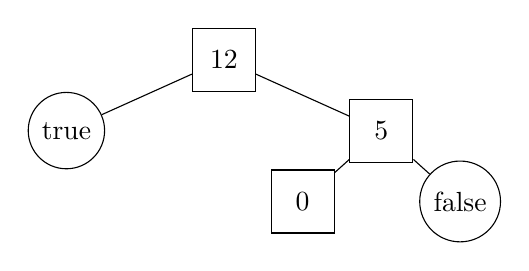
\begin{tikzpicture}[level distance=0.9cm,
    level 1/.style={sibling distance=4cm},
    level 2/.style={sibling distance=2cm},
    level 3/.style={sibling distance=2cm}
    ]
    \node[minimum size=0.8cm, draw] {12}
      child {node[circle, draw] {true}}
      child {node[minimum size=0.8cm, draw] {5}
        child {node[minimum size=0.8cm, draw] {0}}
        child {node[circle, draw] {false}}
      };
  \end{tikzpicture}
  \]
	
	\podnaloga Definirajte funkciji \verb|adepth| in \verb|bdepth| tipa \verb|('a, 'b) tree -> int|, ki vrneta globino najglobljega A oz.\ B vozlišča. Na zgornjem primeru sta torej obe globini enaki 3, če pa vozlišče, ki vsebuje \verb|0|, nadomestimo z novim vozliščem \verb|false|, bi funkcija \verb|adepth| sedaj vrnila 2.
	
	\podnaloga Definirajte zapisni tip \verb|result| in funkcijo \verb|count: ('a, 'b) tree -> result|, ki prešteje število posameznih vozlišč v AB drevesu kot je prikazano v primeru.
	\begin{verbatim}
	# count test;;
	- : result = {aNodes = 3; bNodes = 2}
	\end{verbatim}
	
	\podnaloga Definirajte funkcijo \verb|is_typemirror : ('a, 'b) tree -> ('b, 'a) tree -> bool|, ki preveri, ali sta si drevesi zrcalni v uporabi A in B vozlišč (torej sta matematično gledano enaki, le da prvo drevo uporablja A vozlišča na mestih, kjer drugo drevo uporablja B vozlišča in obratno).
  \begin{verbatim}
  # is_typemirror (ANode (Empty, 1, Empty)) (BNode (Empty, 1, Empty));;	
  - : bool = true
  \end{verbatim}
    
  \podnaloga Napišite funkcijo \verb|foldmap fa fb acc tr| za hkratno zlaganje in preslikanje AB dreves. Funkciji \verb|fa: 'c -> 'a -> 'c * 'd| in \verb|fb: 'c -> 'b -> 'c * 'e| sprejmeta akumulator tipa \verb|'c| in vrednost vozlišča, ter vrneta posodobljen akumulator in novo vrednost vozlišča. Funkcija \verb|foldmap| zloži ti dve funkciji preko AB drevesa \verb|tr : ('a,'b) tree| z začetnim akumulatorjem \verb|acc : 'c|. Kot rezultat vrne par, končno stanje akumulatorja in novo drevo tipa \verb|('d * 'e) tree|, ki vsebuje posodobljene vrednosti vozlišč. Za poenostavitev problema predpostavite, da vrstni red sprehoda po drevesu ni pomemben.
  \begin{verbatim}
  # foldmap test (fun acc x -> (acc+x, 0)) (fun acc b -> (acc-1, ())) 0;;  
  - : int * (int, unit) tree =
  (15, 
   ANode (BNode (Empty, (), Empty), 0,
    ANode (ANode (Empty, 0, Empty), 0, BNode (Empty, (), Empty))))
  \end{verbatim}

  \naloga
  
  \emph{Nalogo lahko rešujete v Pythonu ali OCamlu.}

  \vspace{3mm}
  \noindent
  Napišite funkcijo \verb|f(k, n)|, ki vrne število vseh zaporedij naravnih števil (naravna števila vsebujejo 0) dolžine $n$, ki se začnejo z 0 in v katerih je razlika med zaporednima členoma manjša ali enaka $k$.
  
	
\end{document}